\section{Microbenchmarks}
\label{sec:experiments:microbenchmarks}

Before conducting our designed experiments, we evaluate our experimental setup through several micro benchmarks. The goal of these benchmarks is to measure the impact of our functional benchmark components and experimental environment.


\subsection{Measuring the impact of a multi-node setup}
\label{sec:experiments:microbenchmarks:node-count}

The first micro benchmark that we have conducted compares two experimental environments. In \cref{sec:experiments:design:environment}, we introduced our experimental environment and discussed the cluster configuration that we have use for our experimental evaluation. We discussed that we designed the experiments to be run on a single node cluster to abolish any variance in network latencies. However, this also implies that the benchmark system is running on the same node and this can have an effect on the results of the experiments.

To evaluate the impact of such a cluster configuration we constructed a micro benchmark. In this micro benchmark, we perform an experiment similar to the design of our first experiment, in which we try to find the maximum throughput of our experimental environment. In this experiment, however, we only perform it on an unmeshed (baseline) configuration to simplify and limit any variance a \gls{sm} system can impose and run it for a total duration of 15 minutes. We compare two experimental environments, in which we change the cluster configuration. The first environment has a single node cluster which runs the benchmark system and the target services. The second environment has a two node cluster, one of these nodes runs the benchmark system whereas the other node runs the target service.


\begin{figure}[!t]
    \centering
    
    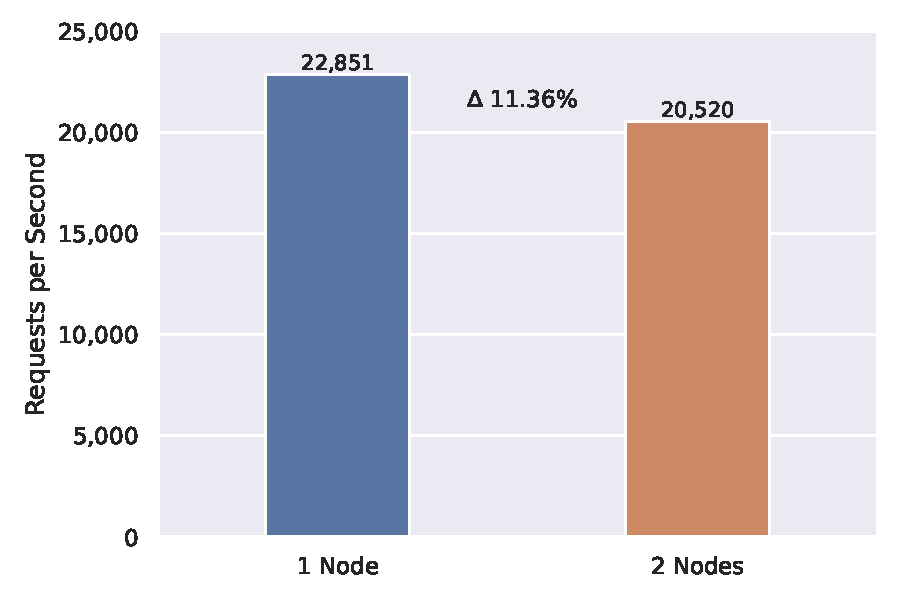
\includegraphics[width=0.8\linewidth]{5_experimental_evaluation/figures/microbench-node-count.pdf}

    \caption[Micro benchmark - Comparing the average maximum throughput of two cluster configurations.]{Comparing the average maximum throughput of two cluster configurations by using an HTTP-based load test in an environment without a service mesh.}
    
    \label{fig:microbench:node-count}
\end{figure}

The results of the micro benchmark can be seen in \cref{fig:microbench:node-count}. The environment using a single node reached an average throughput of 22851 requests per second over the duration of the 15-minute experiment. The environment using two nodes, however, only managed to reach 20520 requests per second. Although the benchmarking system in the two node environment has more system resources to work with, it was unable to reach the throughput levels of the single node environment. Therefore, we can conclude that the experimental environment using one node does not cause any system resource related bottlenecks and that our proposed design using one node is a valid approach for our experiments.


\subsection{Measuring the impact of the impact of our target service}
\label{sec:experiments:microbenchmarks:target-svc}

The second micro benchmark that we conduct tries to establish if the target services can be the cause of a bottleneck during our experimental evaluation. As discussed in our analysis of the \gls{sut} (see \cref{sec:system:sut}), we measure the data path towards our service to evaluate the overheads of a \gls{sm} system and its proxy architecture. However, to evaluate this, we need to emulate a software service that acts as a purely functional component in our benchmark. In our prototype implementation of \textit{Mesh Bench}, we use a simple HTTP and gRPC service (see \cref{sec:system:implementation}). 

To determine if the target service implementation can be the cause of a bottleneck, we used a different workload generator than the one we use for our benchmarking system. Although \textit{fortio} has a flexible feature set and is highly configurable, \textit{wrk2} (as discussed as alternative in \cref{sec:system:implementation}) was the most performant workload generator we have evaluated and can generate more load than the other systems mentioned. During our micro benchmark, we generate several levels of load beyond that of our designed experiments, to make sure that the target service is not a bottleneck in any of the results.

\begin{figure}[!t]
    \centering
    
    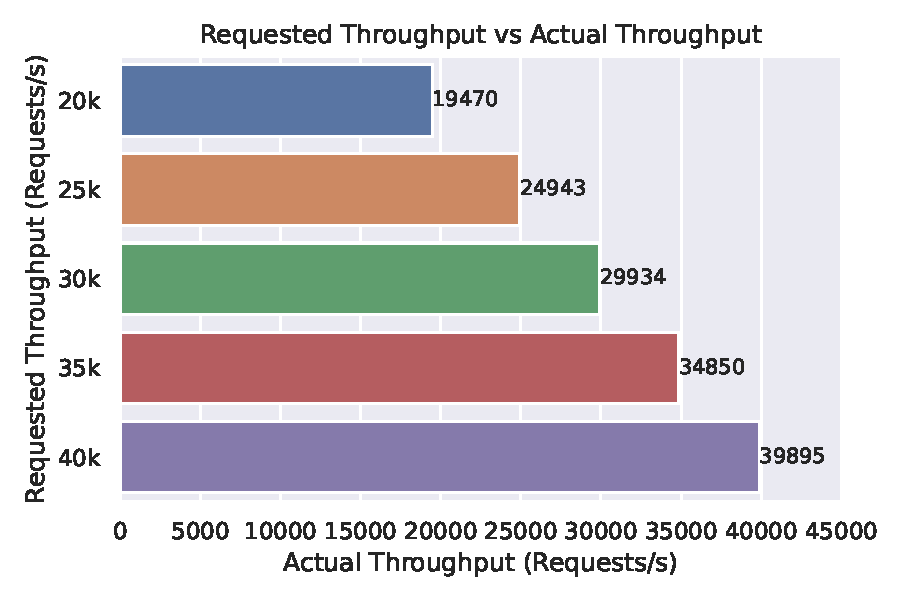
\includegraphics[width=0.8\linewidth]{5_experimental_evaluation/figures/microbench-target-service.pdf}

    \caption[Micro benchmark - Measuring the maximum sustained level of throughput for the target service.]{Measuring the maximum sustained level of throughput for the target service by performing HTTP-based load tests in an environment without a service mesh.}
    
    \label{fig:microbench:target-svc}
\end{figure}

In \cref{fig:microbench:target-svc} we present the results of the micro benchmark. This chart shows the requested throughput of the workload generator on the y-axis and shows the actual throughput of successful requests on the x-axis. From these results, we can derive that the target services had no problems handling the levels of throughput generated as the actual throughput levels are very close to the requested levels. Note that these levels of throughput exceed the maximum throughput of the experiment results as discussed in the next section, which shows that the target service as functional component in our benchmark system is not the cause of any bottlenecks.
